\chapter*{Motivaci\'on}
\addcontentsline{toc}{chapter}{Motivaci\'on y estrategia}
\label{ch:motRadio}

% \textbf{Decir algo del tamanho dle frente de onda y la frecuencia de la radiacion.}

La emisi\'on de radio en lluvias atmosf\'ericas extendidas fue observada por primera vez por Jelley et al.\ en 1964 \cite{jelley1966radio}. Su estudio fue bastante activa durante los a\~nos 70 \cite{allan1971progress}, pero no fue sino hasta las \'ultimas d\'ecadas que los desarrollos en electr\'onica de alta velocidad y en teor\'ia de la informaci\'on permitieron un avance sustancial en el \'area.
Como consecuencia de este resurgimiento se han impulsado varios experimentos que buscan explotar el potencial de la t\'ecnica, como por ejemplo CODALEMA \cite{ardouin2005radio}, LOPES \cite{huege2012lopes}, LOFAR \cite{horandel2009lofar}, Tunka-Rex \cite{schroder2013tunka} o AERA \cite{kelley2011aera}, la extensi\'on de radio del observatorio Pierre Auger.
De esta manera se gener\'o la necesidad de desarrollar nuevas t\'ecnicas de c\'alculo anal\'iticas \cite{huege2003radio,scholten2008macroscopic}, m\'etodos de Monte Carlo \cite{huege2007monte,ludwig2011reas3} o m\'etodos semi-anal\'iticos\cite{scholten2009macroscopic}.

El interés en la técnica reside en que la amplitud del pulso de radio generado en las antenas se encuentra correlacionado con el número de partículas y la energía de la cascada electromagnética, lo que provee información calorimétrica sobre el primario, de manera similar a la técnica de fluorescencia.
Adem\'as, los pulsos almacenados por un arreglo de antenas guardan información sobre el desarrollo longitudinal de la cascada y su $X_{max}$, es decir, son sensibles a la composici\'on de los rayos c\'osmicos primarios \cite{cite:hauge_rec,cite:lofar_rec}.
Finalmente, los arreglos de antenas de radio comparten con los de detectores de partículas sus dos principales ventajas, la reconstrucción de la dirección de arribo se realiza a partir de la medición de tiempos de disparo y su ciclo de trabajo es cercano al \cant{100}{\%}\footnote{por ejemplo, los períodos en los que haya tormentas eléctricas deben descartarse.}.
Todas estas características, sumadas al bajo costo que posee cada antena respecto a los detectores convencionales de partículas hacen de esta técnica de detección una opción competitiva para la próxima generación de detectores de rayos c\'osmicos ultra energ\'eticos.

Esta potencial ganancia en la exposici\'on tambi\'en puede ser aprovechada en la siguiente generaci\'on de detectores de neutrinos ultra energ\'eticos. As\'i, en la actualidad, el proyecto GRAND (Giant Radio Array for Neutrino Detection)~\cite{cite:grand_prop} propone la instalaci\'on de 90000 antenas sobre una superficie de \cant{60000}{km^2} en la cordillera de Tianshan \cite{cite:grand_tec}.
La segunda parte de esta Tesis se dedica precisamente al estudio de las capacidades y limitaciones de un arreglo de superficie de antenas de radio de las caracter\'isticas de GRAND a la hora de detectar neutrinos cósmicos rasantes ultra energéticos.
% Estos números surgen de que la siguiente generación de detectores de superficie requerir\'a aumentar el área cubierta y la cantidad de estaciones respecto del de Auger (que posee el detector de superficie de punta), y al mismo tiempo, mantener la granularidad (distancia entre detectores) con el fin de conservar el nivel de eficiencia a baja energ\'ia (\cant{\sim 10^{17}}{eV}).

\begin{figure}[h!]
	\begin{center}
		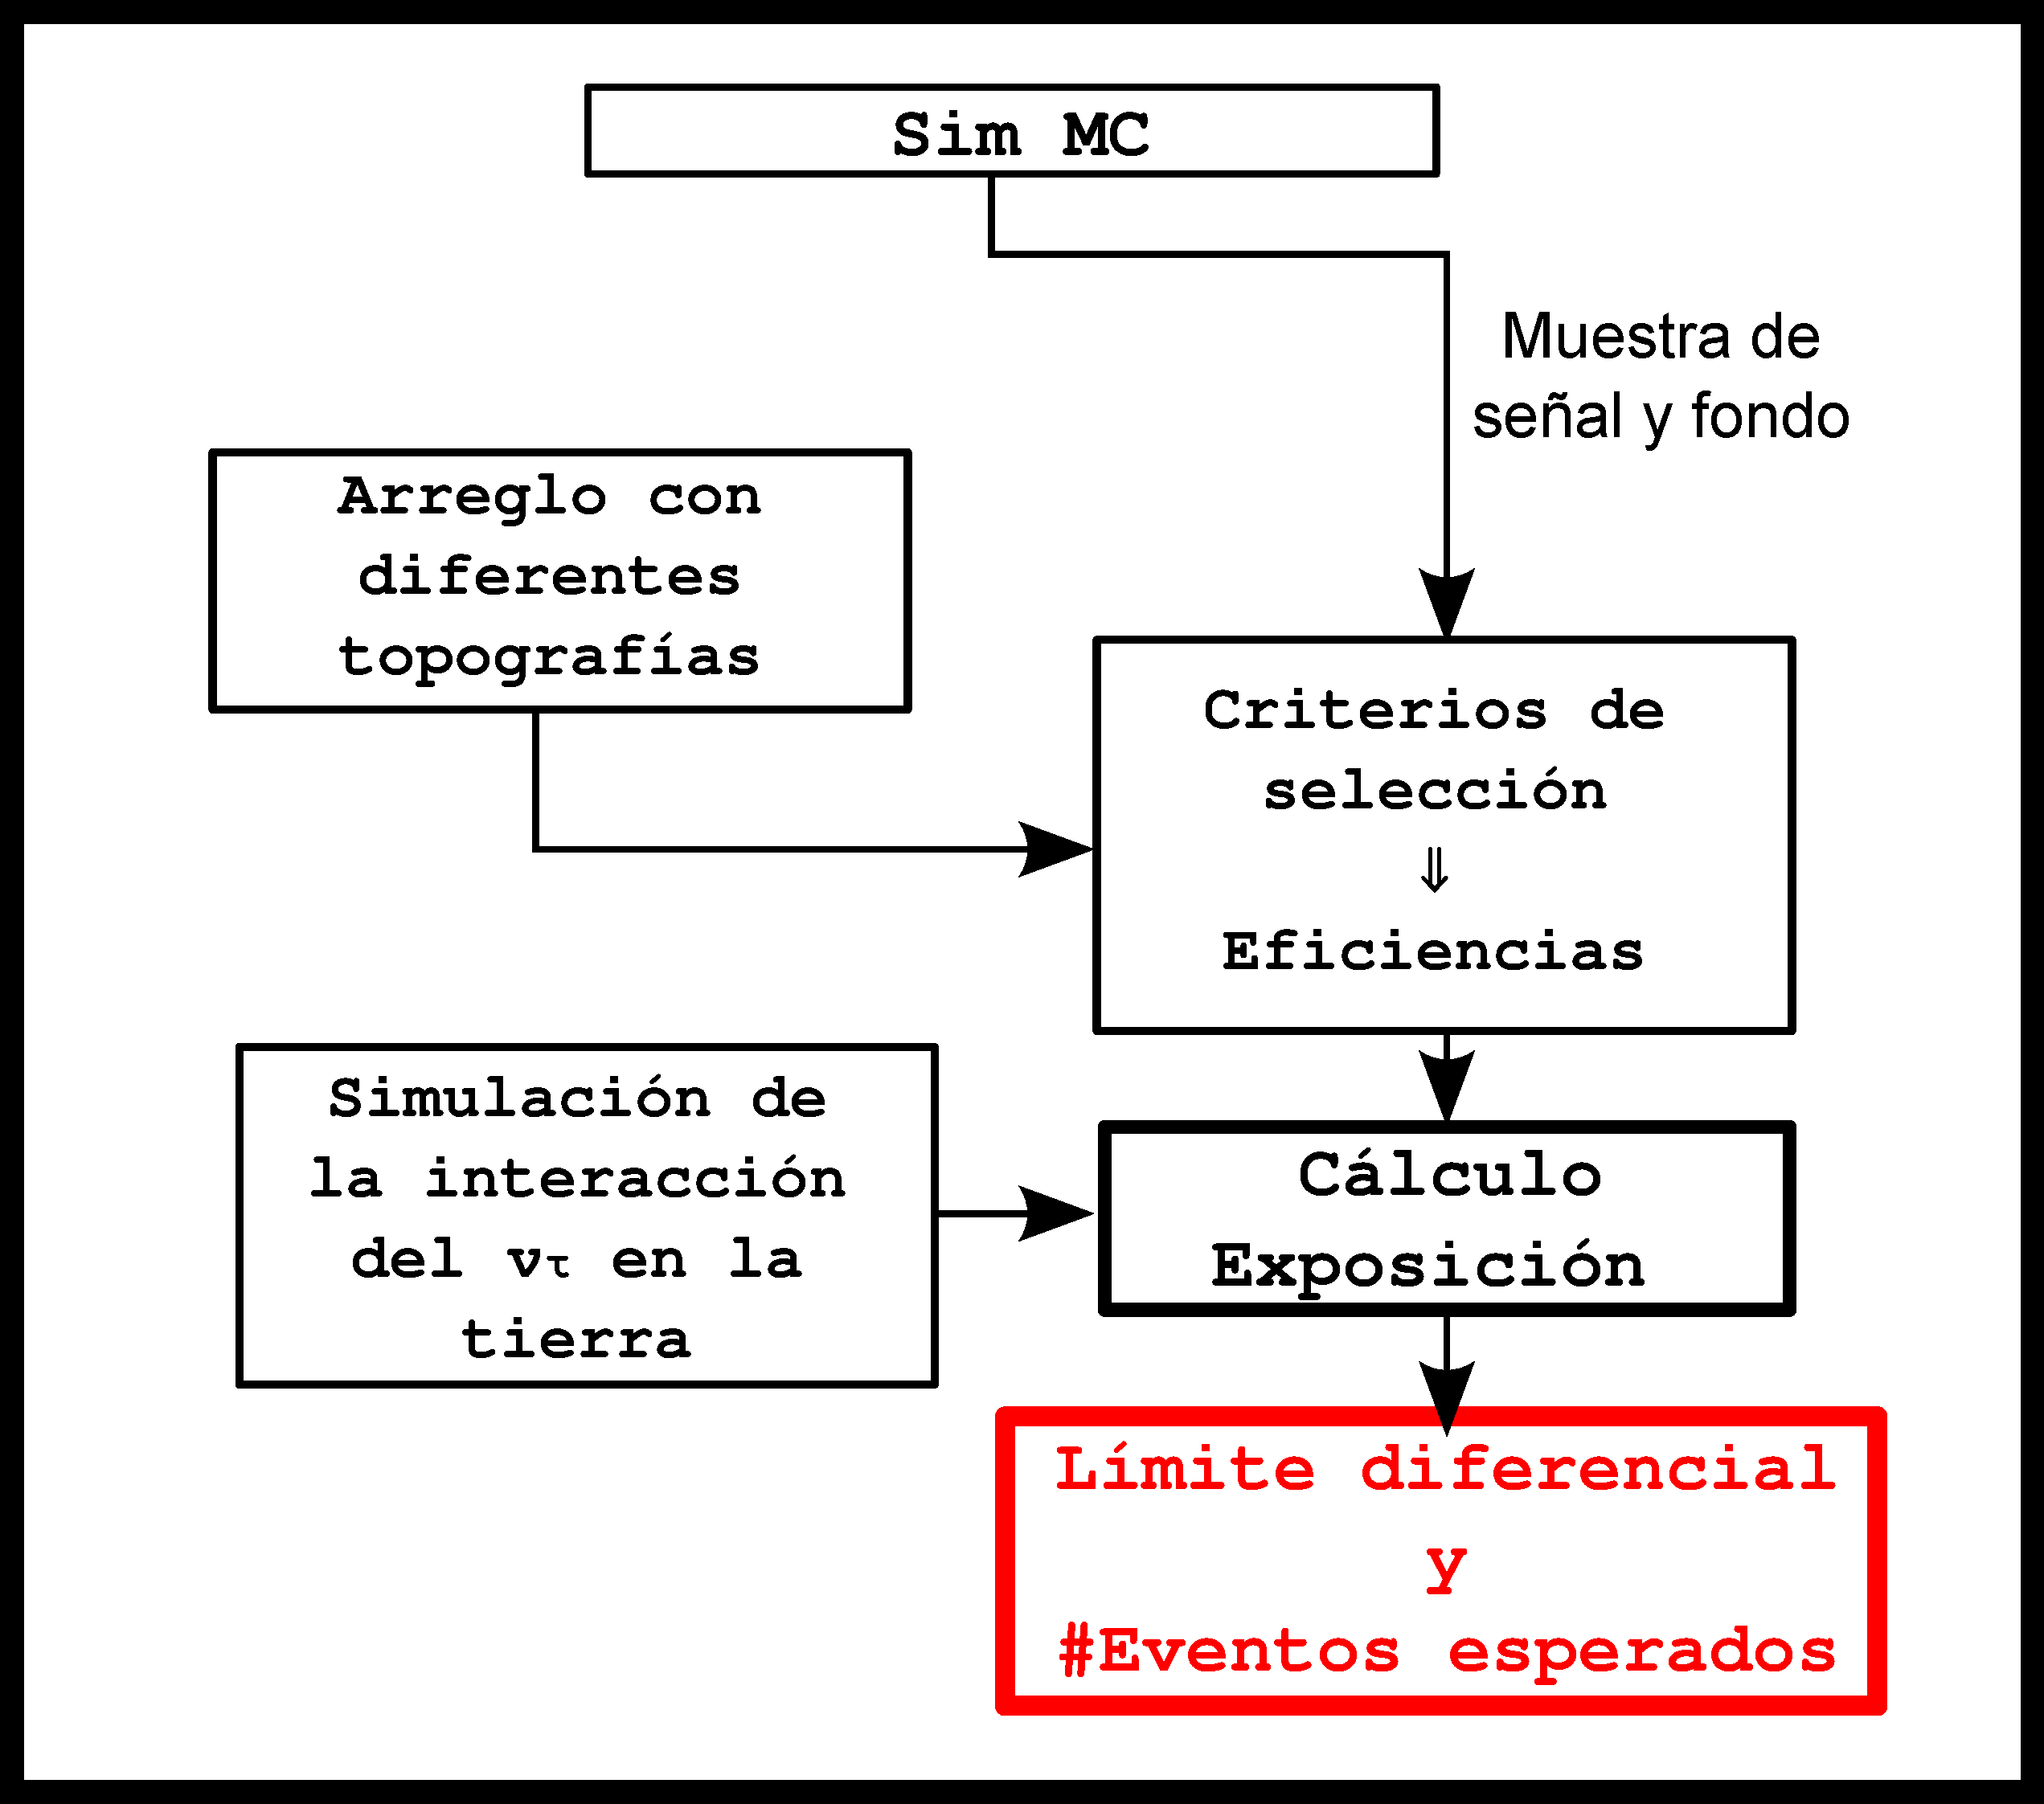
\includegraphics[width=0.9\textwidth]{fig/motivacionRadio/analysisSchemaRadio_v2}
		\caption*{Esquema de la estrategia utilizada para calcular el desempe\~no de un arreglo de antenas. Se utilizaron simulaciones de Monte Carlo de se\~nal y fondo para estudiar criterios de selecci\'on y para determinar las eficiencias de detecci\'on. Estas eficiencias fueron obtenidas para distintas disposiciones alternativas de antenas sobre la superficie. El c\'alculo de la exposici\'on se realiz\'o a trav\'es de un m\'etodo similar al utilizado en Auger. Por \'ultimo, como medida del desempe\~no se reporta el l\'imite diferencial que podr\'ia imponer el detector y el n\'umero de eventos esperados en un tiempo razonable de medici\'on.}
		\label{fig:analysisSchemaRadio}
	\end{center}
\end{figure}
%
Con el fin de calcular el desempe\~no del detector, en esta parte del trabajo se sigui\'o una estrategia inspirada en la utilizada en la b\'usqueda de neutrinos en Auger, que se esquematiza en la Figura.
% \ref{fig:analysisSchemaRadio}.
Una diferencia con el an\'alisis presentado en la Parte I es que, al no existir un dise\~no final del detector, es necesario realizar un conjunto de suposiciones como por ejemplo sobre  su topograf\'ia, cualidades de las antenas, o ubicaci\'on geogr\'afica.
Por otro lado, al no contar con una muestra de datos como representaci\'on del fondo, se utilizaron simulaciones Monte Carlo de eventos hadr\'onicos inclinados.
Tras optimizar los criterios de separaci\'on de se\~nal y fondo, y calcular la exposici\'on del arreglo, se estudi\'o el desempe\~no del detector al variar las caracter\'isticas de las antenas que lo conforman y su disposici\'on sobre la superficie.
Para ello se calcul\'o el l\'imite diferencial que \'este podr\'ia imponer de no observarse se\~nal, y el n\'umero de eventos esperado seg\'un un conjunto de modelos vigentes.

La organizaci\'on de esta segunda parte de la Tesis es la siguiente.
En el capítulo \ref{ch:easRadio} se realiza una introducción a la emisión de radio de las lluvias atmosféricas y se discuten sus características principales, sus mecanismos de producción y un modelo que, mediante hip\'otesis geom\'etricas simplificadas, permite recuperar sus características principales.
En el capítulo \ref{ch:simulacionRadio} se describe la cadena de simulaciones utilizadas para el c\'alculo de la se\~nal en el detector. 
En particular, contiene una revisión detallada de \zhs{}, el programa utilizado para simular la emisión de radio de las EAS.
A continuaci\'om, en el cap\'itulo \ref{ch:caracterizacionRadio} se realiza una caracterización de la señal de radio que generan los neutrinos ES  a nivel del suelo, junto a posibles estrategias para separarlos de las producidos por lluvias hadr\'onicas horizontales.
Finalmente en el capítulo \ref{ch:resultadosRadio} se calculan las eficiencias de disparo e identificaci\'on, la exposición y la sensitividad que podría alcanzar un detector de superficie de 90000 antenas de radio, considerando diferentes topografías.

% \textbf{XXX HACER UN RECUENTO DE LO QUE HAY EN LA SEGUNDA PARTE DE LA TESIS}

